\documentclass[3p]{elsarticle} %review=doublespace preprint=single 5p=2 column
%%% Begin My package additions %%%%%%%%%%%%%%%%%%%
\usepackage[hyphens]{url}

  \journal{DS621 - Homework 3} % Sets Journal name


\usepackage{lineno} % add
\providecommand{\tightlist}{%
  \setlength{\itemsep}{0pt}\setlength{\parskip}{0pt}}

\usepackage{graphicx}
%%%%%%%%%%%%%%%% end my additions to header

\usepackage[T1]{fontenc}
\usepackage{lmodern}
\usepackage{amssymb,amsmath}
\usepackage{ifxetex,ifluatex}
\usepackage{fixltx2e} % provides \textsubscript
% use upquote if available, for straight quotes in verbatim environments
\IfFileExists{upquote.sty}{\usepackage{upquote}}{}
\ifnum 0\ifxetex 1\fi\ifluatex 1\fi=0 % if pdftex
  \usepackage[utf8]{inputenc}
\else % if luatex or xelatex
  \usepackage{fontspec}
  \ifxetex
    \usepackage{xltxtra,xunicode}
  \fi
  \defaultfontfeatures{Mapping=tex-text,Scale=MatchLowercase}
  \newcommand{\euro}{€}
\fi
% use microtype if available
\IfFileExists{microtype.sty}{\usepackage{microtype}}{}
\bibliographystyle{elsarticle-harv}
\usepackage{color}
\usepackage{fancyvrb}
\newcommand{\VerbBar}{|}
\newcommand{\VERB}{\Verb[commandchars=\\\{\}]}
\DefineVerbatimEnvironment{Highlighting}{Verbatim}{commandchars=\\\{\}}
% Add ',fontsize=\small' for more characters per line
\usepackage{framed}
\definecolor{shadecolor}{RGB}{248,248,248}
\newenvironment{Shaded}{\begin{snugshade}}{\end{snugshade}}
\newcommand{\AlertTok}[1]{\textcolor[rgb]{0.94,0.16,0.16}{#1}}
\newcommand{\AnnotationTok}[1]{\textcolor[rgb]{0.56,0.35,0.01}{\textbf{\textit{#1}}}}
\newcommand{\AttributeTok}[1]{\textcolor[rgb]{0.77,0.63,0.00}{#1}}
\newcommand{\BaseNTok}[1]{\textcolor[rgb]{0.00,0.00,0.81}{#1}}
\newcommand{\BuiltInTok}[1]{#1}
\newcommand{\CharTok}[1]{\textcolor[rgb]{0.31,0.60,0.02}{#1}}
\newcommand{\CommentTok}[1]{\textcolor[rgb]{0.56,0.35,0.01}{\textit{#1}}}
\newcommand{\CommentVarTok}[1]{\textcolor[rgb]{0.56,0.35,0.01}{\textbf{\textit{#1}}}}
\newcommand{\ConstantTok}[1]{\textcolor[rgb]{0.00,0.00,0.00}{#1}}
\newcommand{\ControlFlowTok}[1]{\textcolor[rgb]{0.13,0.29,0.53}{\textbf{#1}}}
\newcommand{\DataTypeTok}[1]{\textcolor[rgb]{0.13,0.29,0.53}{#1}}
\newcommand{\DecValTok}[1]{\textcolor[rgb]{0.00,0.00,0.81}{#1}}
\newcommand{\DocumentationTok}[1]{\textcolor[rgb]{0.56,0.35,0.01}{\textbf{\textit{#1}}}}
\newcommand{\ErrorTok}[1]{\textcolor[rgb]{0.64,0.00,0.00}{\textbf{#1}}}
\newcommand{\ExtensionTok}[1]{#1}
\newcommand{\FloatTok}[1]{\textcolor[rgb]{0.00,0.00,0.81}{#1}}
\newcommand{\FunctionTok}[1]{\textcolor[rgb]{0.00,0.00,0.00}{#1}}
\newcommand{\ImportTok}[1]{#1}
\newcommand{\InformationTok}[1]{\textcolor[rgb]{0.56,0.35,0.01}{\textbf{\textit{#1}}}}
\newcommand{\KeywordTok}[1]{\textcolor[rgb]{0.13,0.29,0.53}{\textbf{#1}}}
\newcommand{\NormalTok}[1]{#1}
\newcommand{\OperatorTok}[1]{\textcolor[rgb]{0.81,0.36,0.00}{\textbf{#1}}}
\newcommand{\OtherTok}[1]{\textcolor[rgb]{0.56,0.35,0.01}{#1}}
\newcommand{\PreprocessorTok}[1]{\textcolor[rgb]{0.56,0.35,0.01}{\textit{#1}}}
\newcommand{\RegionMarkerTok}[1]{#1}
\newcommand{\SpecialCharTok}[1]{\textcolor[rgb]{0.00,0.00,0.00}{#1}}
\newcommand{\SpecialStringTok}[1]{\textcolor[rgb]{0.31,0.60,0.02}{#1}}
\newcommand{\StringTok}[1]{\textcolor[rgb]{0.31,0.60,0.02}{#1}}
\newcommand{\VariableTok}[1]{\textcolor[rgb]{0.00,0.00,0.00}{#1}}
\newcommand{\VerbatimStringTok}[1]{\textcolor[rgb]{0.31,0.60,0.02}{#1}}
\newcommand{\WarningTok}[1]{\textcolor[rgb]{0.56,0.35,0.01}{\textbf{\textit{#1}}}}
\usepackage{graphicx}
\ifxetex
  \usepackage[setpagesize=false, % page size defined by xetex
              unicode=false, % unicode breaks when used with xetex
              xetex]{hyperref}
\else
  \usepackage[unicode=true]{hyperref}
\fi
\hypersetup{breaklinks=true,
            bookmarks=true,
            pdfauthor={},
            pdftitle={DS621 - Homework 3},
            colorlinks=false,
            urlcolor=blue,
            linkcolor=magenta,
            pdfborder={0 0 0}}
\urlstyle{same}  % don't use monospace font for urls

\setcounter{secnumdepth}{0}
% Pandoc toggle for numbering sections (defaults to be off)
\setcounter{secnumdepth}{0}

% Pandoc citation processing

% Pandoc header
\usepackage{booktabs}
\usepackage{longtable}
\usepackage{array}
\usepackage{multirow}
\usepackage{wrapfig}
\usepackage{float}
\usepackage{colortbl}
\usepackage{pdflscape}
\usepackage{tabu}
\usepackage{threeparttable}
\usepackage{threeparttablex}
\usepackage[normalem]{ulem}
\usepackage{makecell}
\usepackage{xcolor}



\begin{document}
\begin{frontmatter}

  \title{DS621 - Homework 3}
    \author[Critical Thinking Group 2 - DS621]{George Cruz Deschamps}
   \ead{georg4re@gmail.com} 
    \author[Critical Thinking Group 2 - DS621]{Karim Hammoud}
   \ead{cunykarim@gmail.com} 
    \author[Critical Thinking Group 2 - DS621]{Maliat Islam}
   \ead{maliat.islam21@gmail.com} 
    \author[Critical Thinking Group 2 - DS621]{Matthew Lucich}
   \ead{matt.lucich@gmail.com} 
    \author[Critical Thinking Group 2 - DS621]{Gabriella Martinez}
   \ead{gpmmrtzz@gmail.com} 
    \author[Critical Thinking Group 2 - DS621]{Ken Popkin}
   \ead{krpopkin@gmail.com} 
      
  \begin{abstract}
  In this homework assignment, we will explore, analyze and model a data
  set containing information on crime for various neighborhoods of a major
  city. Each record has a response variable indicating whether or not the
  crime rate is above the median crime rate (1) or not (0).
  \end{abstract}
  
 \end{frontmatter}

Our objective is to build three different binary logistic regression
models on the training data set to predict whether or not neighborhoods
are at risk for high crime. We will provide classifications and
probabilities for the evaluation data set using your binary logistic
regression model. We can only use the variables given (or variables
derived from the variables provided). Below is a short description of
the variables of interest in the data set:

\begin{itemize}
\tightlist
\item
  \texttt{zn} proportion of residential land zoned for lots over 25,000
  sq.ft.
\item
  \texttt{indus} proportion of non-retail business acres per town
\item
  \texttt{chas} Charles River dummy variable (= 1 if tract bounds river;
  0 otherwise)
\item
  \texttt{nox} nitrogen oxides concentration (parts per 10 million)
\item
  \texttt{rm} average number of rooms per dwelling
\item
  \texttt{age} proportion of owner-occupied units built prior to 1940
\item
  \texttt{dis} weighted distances to five Boston employment centers
\item
  \texttt{rad} index of accessibility to radial highways
\item
  \texttt{tax} full-value property-tax rate per \$10,000
\item
  \texttt{ptratio} pupil-teacher ratio by town
\item
  \texttt{lstat} \% lower status of the population
\item
  \texttt{medv} median value of owner-occupied homes in \$1000's
\item
  \texttt{target} indicating whether or not the crime rate is above the
  median crime rate (1) or not (0) \textbf{response variable}
\end{itemize}

\newpage

\hypertarget{the-data}{%
\section{The Data}\label{the-data}}

\hypertarget{data-exploration}{%
\paragraph{Data Exploration}\label{data-exploration}}

Exploratory data analysis is the process to get to know your data, so
that a hypothesis can be generated and later tested. Visualization
techniques are usually applied to aid the exploration of the data.

To get introduced to the dataset, we use DataExplorer's
\texttt{introduce()} function:

\begin{tabular}{l|r}
\hline
  & \\
\hline
rows & 466\\
\hline
columns & 13\\
\hline
discrete\_columns & 0\\
\hline
continuous\_columns & 13\\
\hline
all\_missing\_columns & 0\\
\hline
total\_missing\_values & 0\\
\hline
complete\_rows & 466\\
\hline
total\_observations & 6,058\\
\hline
memory\_usage & 44,440\\
\hline
\end{tabular}

Using dplyr's \texttt{glimpse()}\footnote{https://www.rdocumentation.org/packages/dplyr/versions/0.3/topics/glimpse}
function, we can take a ``glimpse'' into both the \texttt{crime\_train}
and \texttt{crime\_test} data respectively, and easily see the
dimensions, variable names and types.

From this \texttt{glimpse()} into the \texttt{crime\_train} dataset, we
confirm the two variables \texttt{chas} and \texttt{target} are
factors\footnote{https://www.stat.berkeley.edu/\textasciitilde s133/factors.html\#}
as noted in the description of variables above. These variables will be
transformed in our data preparation stage.

\begin{verbatim}
## Rows: 466
## Columns: 13
## $ zn      <dbl> 0, 0, 0, 30, 0, 0, 0, 0, 0, 80, 22, 0, 0, 22, 0, 0, 100, 20, 0~
## $ indus   <dbl> 19.58, 19.58, 18.10, 4.93, 2.46, 8.56, 18.10, 18.10, 5.19, 3.6~
## $ chas    <int> 0, 1, 0, 0, 0, 0, 0, 0, 0, 0, 0, 0, 0, 0, 0, 0, 0, 0, 0, 0, 0,~
## $ nox     <dbl> 0.605, 0.871, 0.740, 0.428, 0.488, 0.520, 0.693, 0.693, 0.515,~
## $ rm      <dbl> 7.929, 5.403, 6.485, 6.393, 7.155, 6.781, 5.453, 4.519, 6.316,~
## $ age     <dbl> 96.2, 100.0, 100.0, 7.8, 92.2, 71.3, 100.0, 100.0, 38.1, 19.1,~
## $ dis     <dbl> 2.0459, 1.3216, 1.9784, 7.0355, 2.7006, 2.8561, 1.4896, 1.6582~
## $ rad     <int> 5, 5, 24, 6, 3, 5, 24, 24, 5, 1, 7, 5, 24, 7, 3, 3, 5, 5, 24, ~
## $ tax     <int> 403, 403, 666, 300, 193, 384, 666, 666, 224, 315, 330, 398, 66~
## $ ptratio <dbl> 14.7, 14.7, 20.2, 16.6, 17.8, 20.9, 20.2, 20.2, 20.2, 16.4, 19~
## $ lstat   <dbl> 3.70, 26.82, 18.85, 5.19, 4.82, 7.67, 30.59, 36.98, 5.68, 9.25~
## $ medv    <dbl> 50.0, 13.4, 15.4, 23.7, 37.9, 26.5, 5.0, 7.0, 22.2, 20.9, 24.8~
## $ target  <int> 1, 1, 1, 0, 0, 0, 1, 1, 0, 0, 0, 0, 1, 1, 0, 0, 0, 1, 1, 1, 0,~
\end{verbatim}

\begin{verbatim}
## Rows: 40
## Columns: 12
## $ zn      <int> 0, 0, 0, 0, 0, 25, 25, 0, 0, 0, 0, 0, 0, 0, 0, 0, 0, 0, 22, 90~
## $ indus   <dbl> 7.07, 8.14, 8.14, 8.14, 5.96, 5.13, 5.13, 4.49, 4.49, 2.89, 25~
## $ chas    <int> 0, 0, 0, 0, 0, 0, 0, 0, 0, 0, 0, 0, 0, 0, 0, 1, 0, 0, 0, 0, 0,~
## $ nox     <dbl> 0.469, 0.538, 0.538, 0.538, 0.499, 0.453, 0.453, 0.449, 0.449,~
## $ rm      <dbl> 7.185, 6.096, 6.495, 5.950, 5.850, 5.741, 5.966, 6.630, 6.121,~
## $ age     <dbl> 61.1, 84.5, 94.4, 82.0, 41.5, 66.2, 93.4, 56.1, 56.8, 69.6, 97~
## $ dis     <dbl> 4.9671, 4.4619, 4.4547, 3.9900, 3.9342, 7.2254, 6.8185, 4.4377~
## $ rad     <int> 2, 4, 4, 4, 5, 8, 8, 3, 3, 2, 2, 2, 4, 5, 5, 4, 8, 8, 7, 1, 1,~
## $ tax     <int> 242, 307, 307, 307, 279, 284, 284, 247, 247, 276, 188, 188, 43~
## $ ptratio <dbl> 17.8, 21.0, 21.0, 21.0, 19.2, 19.7, 19.7, 18.5, 18.5, 18.0, 19~
## $ lstat   <dbl> 4.03, 10.26, 12.80, 27.71, 8.77, 13.15, 14.44, 6.53, 8.44, 11.~
## $ medv    <dbl> 34.7, 18.2, 18.4, 13.2, 21.0, 18.7, 16.0, 26.6, 22.2, 21.4, 17~
\end{verbatim}

Next, we proceed with our exploratory data analysis by providing
univariate descriptive statistics on our training dataset,
\texttt{crime\_train}.

\begin{table}

\caption{\label{tab:unnamed-chunk-2}Univariate Descriptive Statistics - Training Data Set}
\centering
\begin{tabular}[t]{l|r|r|r|r|r|r|r}
\hline
  & Mean & Std.Dev & Min & Q1 & Median & Q3 & Max\\
\hline
age & 68.3675966 & 28.3213784 & 2.9000 & 43.7000 & 77.15000 & 94.1000 & 100.0000\\
\hline
chas & 0.0708155 & 0.2567920 & 0.0000 & 0.0000 & 0.00000 & 0.0000 & 1.0000\\
\hline
dis & 3.7956929 & 2.1069496 & 1.1296 & 2.1007 & 3.19095 & 5.2146 & 12.1265\\
\hline
indus & 11.1050215 & 6.8458549 & 0.4600 & 5.1300 & 9.69000 & 18.1000 & 27.7400\\
\hline
lstat & 12.6314592 & 7.1018907 & 1.7300 & 7.0100 & 11.35000 & 16.9400 & 37.9700\\
\hline
medv & 22.5892704 & 9.2396814 & 5.0000 & 17.0000 & 21.20000 & 25.0000 & 50.0000\\
\hline
nox & 0.5543105 & 0.1166667 & 0.3890 & 0.4480 & 0.53800 & 0.6240 & 0.8710\\
\hline
ptratio & 18.3984979 & 2.1968447 & 12.6000 & 16.9000 & 18.90000 & 20.2000 & 22.0000\\
\hline
rad & 9.5300429 & 8.6859272 & 1.0000 & 4.0000 & 5.00000 & 24.0000 & 24.0000\\
\hline
rm & 6.2906738 & 0.7048513 & 3.8630 & 5.8870 & 6.21000 & 6.6300 & 8.7800\\
\hline
target & 0.4914163 & 0.5004636 & 0.0000 & 0.0000 & 0.00000 & 1.0000 & 1.0000\\
\hline
tax & 409.5021459 & 167.9000887 & 187.0000 & 281.0000 & 334.50000 & 666.0000 & 711.0000\\
\hline
zn & 11.5772532 & 23.3646511 & 0.0000 & 0.0000 & 0.00000 & 17.5000 & 100.0000\\
\hline
\end{tabular}
\end{table}

Furthermore, in the histogram plot below, we see that \texttt{medv}, and
\texttt{rm} are normally distributed. We also note bi-modal distribution
of the variables \texttt{indus}, \texttt{rad} and \texttt{tax}. The rest
of the variables show moderate to high skewness on either side
respectively.

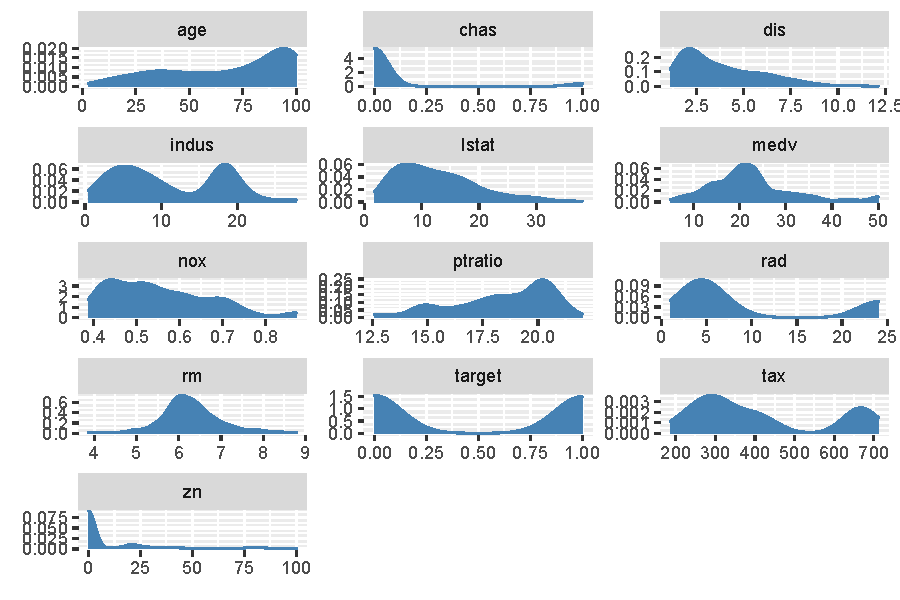
\includegraphics{paper_files/figure-latex/unnamed-chunk-3-1.pdf}

\newpage

In the box-plot figure below, we see many variables exhibit outliers We
also see very high interquartile range for \texttt{rad} and \texttt{tax}
variables where crime rate is above the median. Lastly, the variance
between the 2 values of target differs for \texttt{zn}, \texttt{nox},
\texttt{age}, \texttt{dis}, \texttt{rad} \& \texttt{tax}, which
indicates that we will want to consider adding quadratic terms for them.

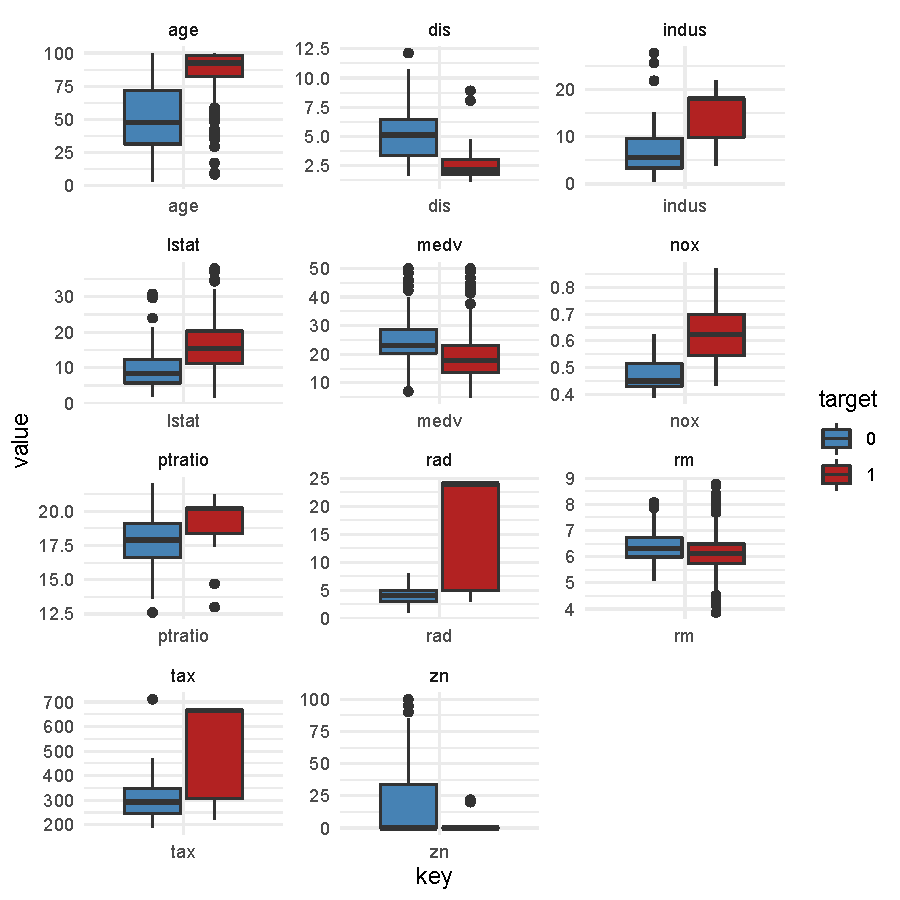
\includegraphics{paper_files/figure-latex/unnamed-chunk-4-1.pdf}

In order to investigate if there is existing correlation between the
data and the target variable, we obtain the values of correlation as
well as a visualization.

\newpage

The correlation table and plot below, we see moderate positive
correlation between variables \texttt{nox}, \texttt{age}, \texttt{rad},
\texttt{tax}, \texttt{indus} and \texttt{target} variables; and moderate
negative correlation between variable dis. And the rest of the variables
have weak or no correlations.

\begin{table}[H]
\centering
\begin{tabular}{l|r}
\hline
  & Correlation\\
\hline
target & 1.0000000\\
\hline
nox & 0.7261062\\
\hline
age & 0.6301062\\
\hline
rad & 0.6281049\\
\hline
tax & 0.6111133\\
\hline
indus & 0.6048507\\
\hline
lstat & 0.4691270\\
\hline
ptratio & 0.2508489\\
\hline
chas & 0.0800419\\
\hline
rm & -0.1525533\\
\hline
medv & -0.2705507\\
\hline
zn & -0.4316818\\
\hline
dis & -0.6186731\\
\hline
\end{tabular}
\end{table}

Below is a correlation matrix of the feature variables in our dataset.
The correlation matrix confirms that multicollinearity is a concern.

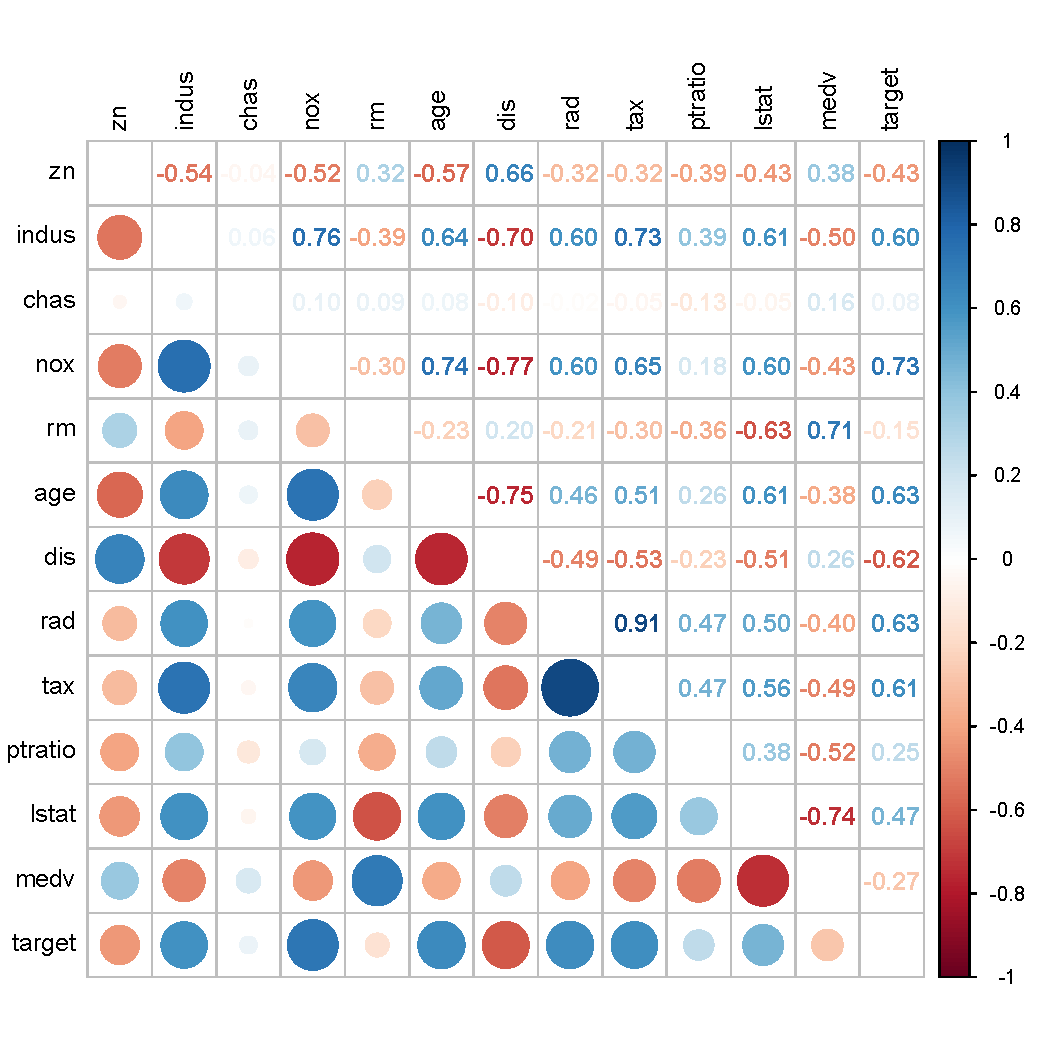
\includegraphics{paper_files/figure-latex/cor-matrix-1.pdf}

\newpage

Lastly, we proceed to check if there are any missing data points in the
\texttt{crime\_train}\textbackslash{}

\begin{tabular}{l|l|l|l|l|l|l|l|l|l|l|l|l}
\hline
zn & indus & chas & nox & rm & age & dis & rad & tax & ptratio & lstat & medv & target\\
\hline
0 & 0 & 0 & 0 & 0 & 0 & 0 & 0 & 0 & 0 & 0 & 0 & 0\\
\hline
\end{tabular}

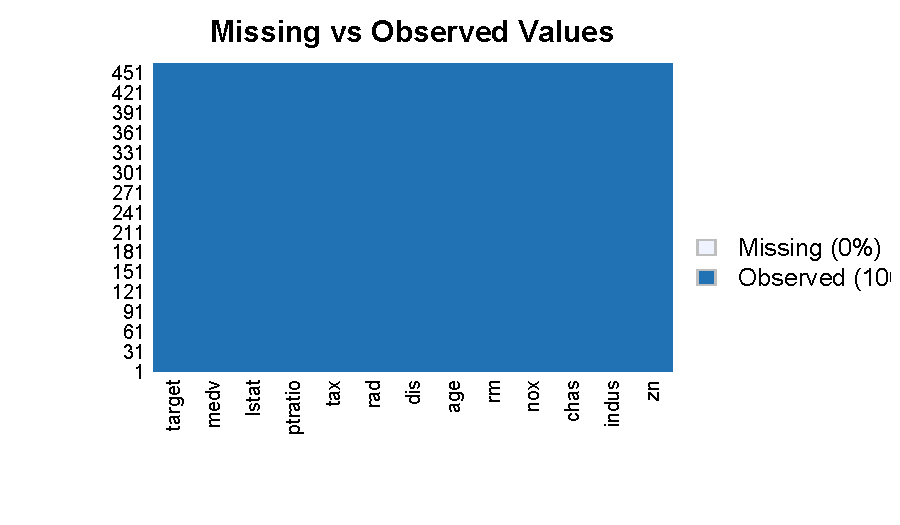
\includegraphics{paper_files/figure-latex/missing-values-1.pdf}

\newpage

\hypertarget{data-preparation}{%
\subsubsection{Data Preparation}\label{data-preparation}}

\textbf{Feature Engineering}\\
In an effort to fine tune our model, we will introduce the use of
feature engineering on select variables.

\begin{itemize}
\tightlist
\item
  \texttt{ptratio\_indicator} assigned a value of 1 if the pupil to
  teacher ratio is \textgreater{} 16, 0 if \texttt{ptratio} is greater
  than 16\footnote{https://www.publicschoolreview.com/average-student-teacher-ratio-stats/national-data}\\
\item
  \texttt{lstat\_indicator} assigned a value of 1 if \textgreater{} 15
  \% of the population is considered low status, 0 otherwise
\item
  \texttt{dis\_indicator} assigned a value of 1 if the distance from
  employment centers is \textgreater{} 4, 0 if \texttt{dis} is less than
  4 (mean value: 3.8)
\end{itemize}

\begin{verbatim}
## 'data.frame':    466 obs. of  17 variables:
##  $ zn                 : num  0 0 0 30 0 0 0 0 0 80 ...
##  $ indus              : num  19.58 19.58 18.1 4.93 2.46 ...
##  $ chas               : Factor w/ 2 levels "0","1": 1 2 1 1 1 1 1 1 1 1 ...
##  $ nox                : num  0.605 0.871 0.74 0.428 0.488 0.52 0.693 0.693 0.515 0.392 ...
##  $ rm                 : num  7.93 5.4 6.49 6.39 7.16 ...
##  $ age                : num  96.2 100 100 7.8 92.2 71.3 100 100 38.1 19.1 ...
##  $ dis                : num  2.05 1.32 1.98 7.04 2.7 ...
##  $ rad                : int  5 5 24 6 3 5 24 24 5 1 ...
##  $ tax                : int  403 403 666 300 193 384 666 666 224 315 ...
##  $ ptratio            : num  14.7 14.7 20.2 16.6 17.8 20.9 20.2 20.2 20.2 16.4 ...
##  $ lstat              : num  3.7 26.82 18.85 5.19 4.82 ...
##  $ medv               : num  50 13.4 15.4 23.7 37.9 26.5 5 7 22.2 20.9 ...
##  $ target             : Factor w/ 2 levels "0","1": 2 2 2 1 1 1 2 2 1 1 ...
##  $ ptratio_indicator  : Factor w/ 2 levels "0","1": 2 2 1 1 1 1 1 1 1 1 ...
##  $ lstat_indicator    : Factor w/ 2 levels "0","1": 2 1 1 2 2 2 1 1 2 2 ...
##  $ dis_indicator      : Factor w/ 2 levels "0","1": 2 2 2 1 2 2 2 2 1 1 ...
##  $ age_greater_than_77: Factor w/ 2 levels "0","1": 2 2 2 1 2 1 2 2 1 1 ...
\end{verbatim}

\newpage

\hypertarget{data-transformation}{%
\subsubsection{Data Transformation}\label{data-transformation}}

Some of the variables are skewed, have outliers or follow a bi-modal
distribution. Therefore, we will perform transformation on some of these
variables. First, we will remove the variable \texttt{tax} due to
multicollinearity and it's high VIF score. Next, we will take log()
transformation of \texttt{age} and \texttt{lstat} variables to lower
skewness. Lastly, we will add quadratic term to \texttt{zn},
\texttt{rad}, and \texttt{nox} variables to account for its variances
with respect to target variable.

\begin{table}[H]
\centering
\begin{tabular}{l|r}
\hline
  & VIF Score\\
\hline
zn & 2.324259\\
\hline
indus & 4.120699\\
\hline
chas & 1.090265\\
\hline
nox & 4.505049\\
\hline
rm & 2.354788\\
\hline
age & 3.134015\\
\hline
dis & 4.240618\\
\hline
rad & 6.781354\\
\hline
tax & 9.217228\\
\hline
ptratio & 2.013109\\
\hline
lstat & 3.649059\\
\hline
medv & 3.667370\\
\hline
\end{tabular}
\end{table}

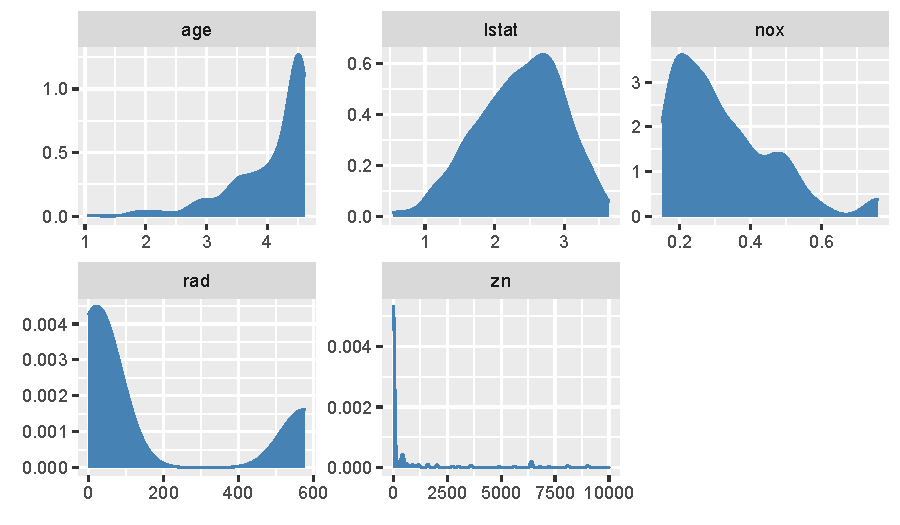
\includegraphics{paper_files/figure-latex/unnamed-chunk-9-1.pdf}

\begin{verbatim}
## 'data.frame':    466 obs. of  16 variables:
##  $ zn                 : num  0 0 0 900 0 0 0 0 0 6400 ...
##  $ indus              : num  19.58 19.58 18.1 4.93 2.46 ...
##  $ chas               : Factor w/ 2 levels "0","1": 1 2 1 1 1 1 1 1 1 1 ...
##  $ nox                : 'AsIs' num  0.366025 0.758641   0.5476 0.183184 0.238144 ...
##  $ rm                 : num  7.93 5.4 6.49 6.39 7.16 ...
##  $ age                : num  4.57 4.61 4.61 2.05 4.52 ...
##  $ dis                : num  2.05 1.32 1.98 7.04 2.7 ...
##  $ rad                : num  25 25 576 36 9 25 576 576 25 1 ...
##  $ ptratio            : num  14.7 14.7 20.2 16.6 17.8 20.9 20.2 20.2 20.2 16.4 ...
##  $ lstat              : num  1.31 3.29 2.94 1.65 1.57 ...
##  $ medv               : num  50 13.4 15.4 23.7 37.9 26.5 5 7 22.2 20.9 ...
##  $ target             : Factor w/ 2 levels "0","1": 2 2 2 1 1 1 2 2 1 1 ...
##  $ ptratio_indicator  : Factor w/ 2 levels "0","1": 2 2 1 1 1 1 1 1 1 1 ...
##  $ lstat_indicator    : Factor w/ 2 levels "0","1": 2 1 1 2 2 2 1 1 2 2 ...
##  $ dis_indicator      : Factor w/ 2 levels "0","1": 2 2 2 1 2 2 2 2 1 1 ...
##  $ age_greater_than_77: Factor w/ 2 levels "0","1": 2 2 2 1 2 1 2 2 1 1 ...
\end{verbatim}

\newpage

\hypertarget{building-the-models}{%
\section{Building the Models}\label{building-the-models}}

First, we begin by building the null binary regression model. We will
use this model to compare it to the subsequent models we build.

Coefficients for the null or Intercept only model:

\begin{verbatim}
## 
## Call:
## glm(formula = target ~ 1, family = binomial(link = "logit"), 
##     data = train)
## 
## Deviance Residuals: 
##    Min      1Q  Median      3Q     Max  
## -1.163  -1.163  -1.163   1.192   1.192  
## 
## Coefficients:
##             Estimate Std. Error z value Pr(>|z|)
## (Intercept) -0.03434    0.09266  -0.371    0.711
## 
## (Dispersion parameter for binomial family taken to be 1)
## 
##     Null deviance: 645.88  on 465  degrees of freedom
## Residual deviance: 645.88  on 465  degrees of freedom
## AIC: 647.88
## 
## Number of Fisher Scoring iterations: 3
\end{verbatim}

\hypertarget{first-model}{%
\subsubsection{First Model}\label{first-model}}

Next we proceed to make our first model using the both the original,
untransformed variables and the engineered features.

\begin{verbatim}
## 
## Call:
## glm(formula = target ~ ., family = binomial(link = "logit"), 
##     data = train)
## 
## Deviance Residuals: 
##     Min       1Q   Median       3Q      Max  
## -1.8917  -0.1328  -0.0010   0.0024   3.5163  
## 
## Coefficients:
##                        Estimate Std. Error z value Pr(>|z|)    
## (Intercept)          -42.873132   7.814964  -5.486 4.11e-08 ***
## zn                    -0.078825   0.038257  -2.060 0.039360 *  
## indus                 -0.062726   0.049280  -1.273 0.203072    
## chas1                  1.059049   0.763475   1.387 0.165398    
## nox                   44.583700   8.718567   5.114 3.16e-07 ***
## rm                    -0.567530   0.745600  -0.761 0.446555    
## age                    0.019072   0.018456   1.033 0.301411    
## dis                    0.666568   0.327609   2.035 0.041887 *  
## rad                    0.745172   0.177312   4.203 2.64e-05 ***
## tax                   -0.007360   0.003288  -2.238 0.025213 *  
## ptratio                0.626502   0.188187   3.329 0.000871 ***
## lstat                  0.078997   0.075812   1.042 0.297405    
## medv                   0.181089   0.071225   2.543 0.011006 *  
## ptratio_indicator1     1.803413   1.156048   1.560 0.118764    
## lstat_indicator1       0.492508   0.686231   0.718 0.472942    
## dis_indicator1         0.296323   0.734391   0.403 0.686584    
## age_greater_than_771   0.655696   0.683259   0.960 0.337226    
## ---
## Signif. codes:  0 '***' 0.001 '**' 0.01 '*' 0.05 '.' 0.1 ' ' 1
## 
## (Dispersion parameter for binomial family taken to be 1)
## 
##     Null deviance: 645.88  on 465  degrees of freedom
## Residual deviance: 187.56  on 449  degrees of freedom
## AIC: 221.56
## 
## Number of Fisher Scoring iterations: 9
\end{verbatim}

The following lists the Marginal Model Plots for \emph{Model 1}:

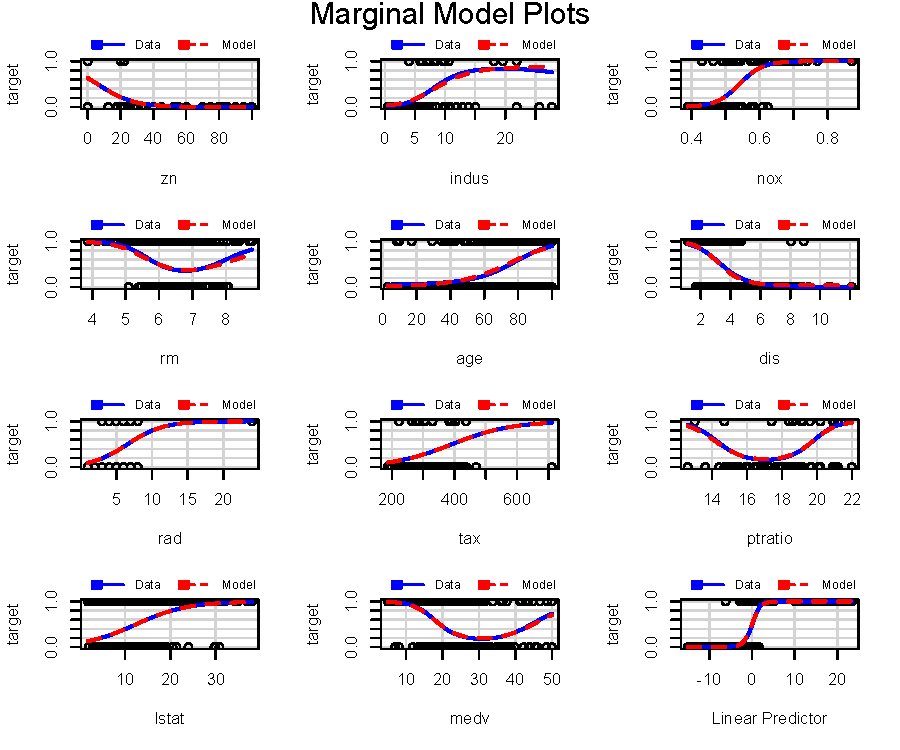
\includegraphics{paper_files/figure-latex/unnamed-chunk-13-1.pdf}

Although the plot appears to hint at a good fit, certain variables seem
to have many outliers which hint at weaker relationships. Several of
these are cubic or quadratic and two of these variables(the
\emph{proportion of landzones} and \emph{distance to employment
centers}) have a negative relationship.

Next, we take a look at the confidence intervals for the regression
coefficients:

\begin{verbatim}
##                             2.5 %        97.5 %
## (Intercept)          -58.19018108 -27.556083221
## zn                    -0.15380693  -0.003842606
## indus                 -0.15931427   0.033861437
## chas1                 -0.43733469   2.555432086
## nox                   27.49562301  61.671777219
## rm                    -2.02887961   0.893820505
## age                   -0.01710002   0.055244413
## dis                    0.02446530   1.308670937
## rad                    0.39764649   1.092698161
## tax                   -0.01380474  -0.000914667
## ptratio                0.25766289   0.995341208
## lstat                 -0.06959190   0.227586891
## medv                   0.04149092   0.320686330
## ptratio_indicator1    -0.46239913   4.069225818
## lstat_indicator1      -0.85247956   1.837495043
## dis_indicator1        -1.14305613   1.735703034
## age_greater_than_771  -0.68346653   1.994858485
\end{verbatim}

\begin{verbatim}
##                                OR        2.5 %       97.5 %
## (Intercept)          2.401238e-19 5.349651e-26 1.077817e-12
## zn                   9.242019e-01 8.574376e-01 9.961648e-01
## indus                9.392004e-01 8.527283e-01 1.034441e+00
## chas1                2.883626e+00 6.457553e-01 1.287686e+01
## nox                  2.303854e+19 8.733682e+11 6.077326e+26
## rm                   5.669243e-01 1.314828e-01 2.444451e+00
## age                  1.019255e+00 9.830454e-01 1.056799e+00
## dis                  1.947542e+00 1.024767e+00 3.701251e+00
## rad                  2.106804e+00 1.488318e+00 2.982310e+00
## tax                  9.926673e-01 9.862901e-01 9.990858e-01
## ptratio              1.871054e+00 1.293903e+00 2.705647e+00
## lstat                1.082202e+00 9.327744e-01 1.255567e+00
## medv                 1.198521e+00 1.042364e+00 1.378073e+00
## ptratio_indicator1   6.070332e+00 6.297709e-01 5.851165e+01
## lstat_indicator1     1.636415e+00 4.263564e-01 6.280785e+00
## dis_indicator1       1.344905e+00 3.188431e-01 5.672915e+00
## age_greater_than_771 1.926483e+00 5.048638e-01 7.351163e+00
\end{verbatim}

The odds ratio would indicate the multiplicative change in odds of crime
for every one unit increase on a predictor variable.\\
\textbf{Odds-ratios for coefficients:}

\begin{verbatim}
##          (Intercept)                   zn                indus 
##         2.401238e-19         9.242019e-01         9.392004e-01 
##                chas1                  nox                   rm 
##         2.883626e+00         2.303854e+19         5.669243e-01 
##                  age                  dis                  rad 
##         1.019255e+00         1.947542e+00         2.106804e+00 
##                  tax              ptratio                lstat 
##         9.926673e-01         1.871054e+00         1.082202e+00 
##                 medv   ptratio_indicator1     lstat_indicator1 
##         1.198521e+00         6.070332e+00         1.636415e+00 
##       dis_indicator1 age_greater_than_771 
##         1.344905e+00         1.926483e+00
\end{verbatim}

\hypertarget{second-model}{%
\subsubsection{Second Model}\label{second-model}}

For our second model, we will use the \texttt{trans\_train} dataset
which includes the transformed variables in the previous section in
addition to the engineered features.

\begin{verbatim}
## 
## Call:
## glm(formula = target ~ ., family = binomial(link = "logit"), 
##     data = trans_train)
## 
## Deviance Residuals: 
##     Min       1Q   Median       3Q      Max  
## -2.0936  -0.1954   0.0000   0.0000   3.3461  
## 
## Coefficients:
##                        Estimate Std. Error z value Pr(>|z|)    
## (Intercept)          -24.446684   6.912815  -3.536 0.000406 ***
## zn                    -0.003352   0.001694  -1.979 0.047854 *  
## indus                 -0.131736   0.049064  -2.685 0.007254 ** 
## chas1                  1.556410   0.761120   2.045 0.040865 *  
## nox                   41.581269   7.974850   5.214 1.85e-07 ***
## rm                    -0.842981   0.697236  -1.209 0.226650    
## age                   -0.038224   0.667053  -0.057 0.954304    
## dis                    0.571657   0.301933   1.893 0.058315 .  
## rad                    0.055708   0.013966   3.989 6.64e-05 ***
## ptratio                0.535961   0.176198   3.042 0.002352 ** 
## lstat                  0.164198   0.799817   0.205 0.837342    
## medv                   0.177604   0.064275   2.763 0.005724 ** 
## ptratio_indicator1     1.408573   1.082973   1.301 0.193377    
## lstat_indicator1       0.066430   0.565626   0.117 0.906507    
## dis_indicator1         0.004908   0.720640   0.007 0.994566    
## age_greater_than_771   1.342623   0.565052   2.376 0.017497 *  
## ---
## Signif. codes:  0 '***' 0.001 '**' 0.01 '*' 0.05 '.' 0.1 ' ' 1
## 
## (Dispersion parameter for binomial family taken to be 1)
## 
##     Null deviance: 645.88  on 465  degrees of freedom
## Residual deviance: 195.16  on 450  degrees of freedom
## AIC: 227.16
## 
## Number of Fisher Scoring iterations: 10
\end{verbatim}

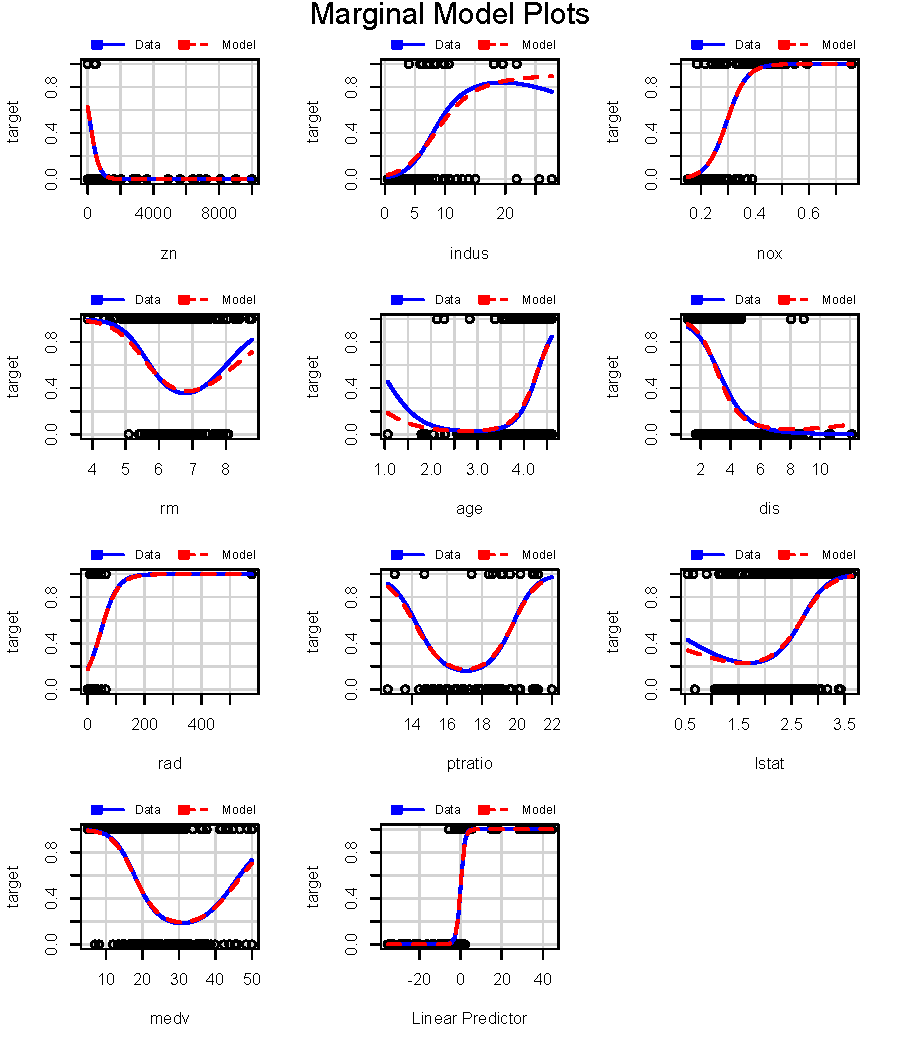
\includegraphics{paper_files/figure-latex/unnamed-chunk-17-1.pdf}

This plot looks very similar to model\_1's, with fewer outliers and
stronger relationships between the data and the model.

\newpage

\hypertarget{third-model}{%
\subsubsection{Third Model}\label{third-model}}

For our third model, we will use some of the original variables:

\begin{verbatim}
## 
## Call:
## glm(formula = target ~ . - rm - chas - age - indus, family = binomial(link = "logit"), 
##     data = trans_train_mod_3)
## 
## Deviance Residuals: 
##     Min       1Q   Median       3Q      Max  
## -2.1908  -0.2806   0.0000   0.0000   3.0407  
## 
## Coefficients:
##               Estimate Std. Error z value Pr(>|z|)    
## (Intercept) -22.812101   4.437941  -5.140 2.74e-07 ***
## zn           -0.003397   0.001442  -2.355  0.01850 *  
## nox          34.818425   5.399202   6.449 1.13e-10 ***
## dis           0.554423   0.190879   2.905  0.00368 ** 
## rad           0.052140   0.011910   4.378 1.20e-05 ***
## ptratio       0.236630   0.099364   2.381  0.01724 *  
## lstat         0.750120   0.560658   1.338  0.18092    
## medv          0.133242   0.042226   3.155  0.00160 ** 
## ---
## Signif. codes:  0 '***' 0.001 '**' 0.01 '*' 0.05 '.' 0.1 ' ' 1
## 
## (Dispersion parameter for binomial family taken to be 1)
## 
##     Null deviance: 645.88  on 465  degrees of freedom
## Residual deviance: 215.94  on 458  degrees of freedom
## AIC: 231.94
## 
## Number of Fisher Scoring iterations: 10
\end{verbatim}

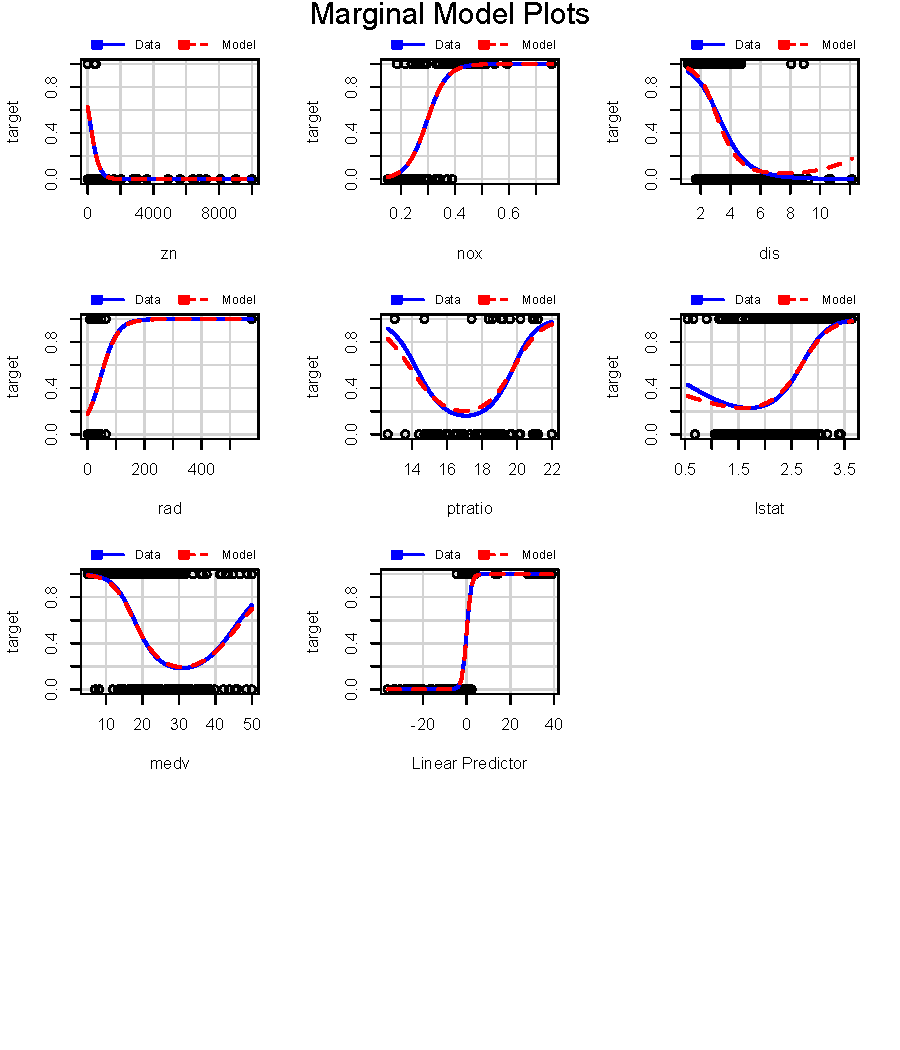
\includegraphics{paper_files/figure-latex/unnamed-chunk-19-1.pdf}

Based on the Marginal model plot, model3 might be the best fit for our
data.

\newpage

\hypertarget{select-models}{%
\section{Select Models}\label{select-models}}

To determine if the models produced have significant improvement in fit
over the null model, we make use of the \texttt{anova()} function.

\begin{verbatim}
## Analysis of Deviance Table
## 
## Model 1: target ~ 1
## Model 2: target ~ zn + indus + chas + nox + rm + age + dis + rad + tax + 
##     ptratio + lstat + medv + ptratio_indicator + lstat_indicator + 
##     dis_indicator + age_greater_than_77
## Model 3: target ~ zn + indus + chas + nox + rm + age + dis + rad + ptratio + 
##     lstat + medv + ptratio_indicator + lstat_indicator + dis_indicator + 
##     age_greater_than_77
## Model 4: target ~ (zn + indus + chas + nox + rm + age + dis + rad + ptratio + 
##     lstat + medv) - rm - chas - age - indus
##   Resid. Df Resid. Dev Df Deviance  Pr(>Chi)    
## 1       465     645.88                          
## 2       449     187.56 16   458.32 < 2.2e-16 ***
## 3       450     195.16 -1    -7.60  0.005845 ** 
## 4       458     215.94 -8   -20.78  0.007747 ** 
## ---
## Signif. codes:  0 '***' 0.001 '**' 0.01 '*' 0.05 '.' 0.1 ' ' 1
\end{verbatim}

The Akaike information criterion (AIC) is a good test for model fit. AIC
calculates the information value of each model by balancing the
variation explained against the number of parameters used.

In AIC model selection, we compare the information value of each model
and choose the one with the lowest AIC value (a lower number means more
information explained!)

\begin{verbatim}
## 
## Model selection based on AICc:
## 
##         K   AICc Delta_AICc AICcWt Cum.Wt      LL
## model1 17 222.92       0.00   0.93   0.93  -93.78
## model2 16 228.37       5.44   0.06   0.99  -97.58
## model3  8 232.25       9.33   0.01   1.00 -107.97
\end{verbatim}

\hypertarget{conclusions}{%
\subsubsection{Conclusions}\label{conclusions}}

We fitted three models using a combination of variables/strategies:
original, engineered and removing certain variables. We looked at the
marginal model plots as well as the Akaike Information Criterion. Since
for the AIC a lower number means more information explained, we have
chosen Model3 as the best fit model.

\newpage

\hypertarget{references}{%
\section{References}\label{references}}

Minitab Support, Accessed 10/2021: ``Interpret the key results for
Marginal Plot''
{[}https://support.minitab.com/en-us/minitab/19/help-and-how-to/graphs/marginal-plot/interpret-the-results/key-results/{]}

Research compendium cboettig/noise-phenomena: Supplement to: ``From
noise to knowledge: how randomness generates novel phenomena and reveals
information'' by Carl Boettiger

Yogita Bor, Accessed 10/2021: Guide for building an End-to-End Logistic
Regression Model.
{[}https://www.analyticsvidhya.com/blog/2021/09/guide-for-building-an-end-to-end-logistic-regression-model/?utm\_source=feedburner\&utm\_medium=email\&utm\_campaign=Feed\%3A+AnalyticsVidhya+\%28Analytics+Vidhya\%29{]}

\newpage

\hypertarget{appendix-a-code}{%
\section{Appendix A: Code}\label{appendix-a-code}}

\begin{Shaded}
\begin{Highlighting}[]
\CommentTok{#load data}
\NormalTok{crime_train <-}\StringTok{ }\KeywordTok{read.csv}\NormalTok{(}\KeywordTok{paste}\NormalTok{(}\StringTok{"https://raw.githubusercontent.com"}\NormalTok{,}
                      \StringTok{"/akarimhammoud/Data_621/main/Assignment_3/"}\NormalTok{,}
                      \StringTok{"data/crime-training-data_modified.csv"}\NormalTok{))}
\NormalTok{crime_test <-}\StringTok{ }\KeywordTok{read.csv}\NormalTok{(}\KeywordTok{paste}\NormalTok{(}\StringTok{"https://raw.githubusercontent.com"}\NormalTok{,}
                       \StringTok{"/akarimhammoud/Data_621/main/Assignment_3/"}\NormalTok{,}
                       \StringTok{"data/crime-evaluation-data_modified.csv"}\NormalTok{))}
\end{Highlighting}
\end{Shaded}

\begin{Shaded}
\begin{Highlighting}[]
\CommentTok{# Data Exploration }
\KeywordTok{descr}\NormalTok{(crime_train,}
  \DataTypeTok{headings =} \OtherTok{FALSE}\NormalTok{, }\CommentTok{#remove headings# }
  \DataTypeTok{transpose =} \OtherTok{TRUE} \CommentTok{#allows for better display due to large amount of variables}
\NormalTok{  ) }\OperatorTok\StringTok{ }
\StringTok{  }\KeywordTok{kbl}\NormalTok{(}\DataTypeTok{caption =} \StringTok{"Univariate Descriptive Statistics - Training Data Set"}\NormalTok{) }\OperatorTok
\StringTok{  }\KeywordTok{kable_styling}\NormalTok{(}\DataTypeTok{bootstrap_options =} \KeywordTok{c}\NormalTok{(}\StringTok{"striped"}\NormalTok{, }\StringTok{"hover"}\NormalTok{, }\StringTok{"condensed"}\NormalTok{))}
\end{Highlighting}
\end{Shaded}

\begin{Shaded}
\begin{Highlighting}[]
\CommentTok{# distribution of the varaibles}
\NormalTok{crime_train }\OperatorTok\StringTok{ }
\StringTok{  }\KeywordTok{gather}\NormalTok{(variable, value, zn}\OperatorTok{:}\NormalTok{target) }\OperatorTok
\StringTok{  }\KeywordTok{ggplot}\NormalTok{(., }\KeywordTok{aes}\NormalTok{(value)) }\OperatorTok{+}\StringTok{ }
\StringTok{  }\KeywordTok{geom_density}\NormalTok{(}\DataTypeTok{fill =} \StringTok{"steelblue"}\NormalTok{, }\DataTypeTok{color=}\StringTok{"steelblue"}\NormalTok{) }\OperatorTok{+}\StringTok{ }
\StringTok{  }\KeywordTok{facet_wrap}\NormalTok{(}\OperatorTok{~}\NormalTok{variable, }\DataTypeTok{scales =}\StringTok{"free"}\NormalTok{, }\DataTypeTok{ncol =} \DecValTok{4}\NormalTok{) }\OperatorTok{+}
\StringTok{  }\KeywordTok{labs}\NormalTok{(}\DataTypeTok{x =} \KeywordTok{element_blank}\NormalTok{(), }\DataTypeTok{y =} \KeywordTok{element_blank}\NormalTok{())}
\end{Highlighting}
\end{Shaded}

\begin{Shaded}
\begin{Highlighting}[]
\CommentTok{# Check for NA values}
\KeywordTok{map}\NormalTok{(crime_train, }\OperatorTok{~}\KeywordTok{sum}\NormalTok{(}\KeywordTok{is.na}\NormalTok{(.))) }\OperatorTok\StringTok{ }\KeywordTok{t}\NormalTok{()}
\end{Highlighting}
\end{Shaded}

\begin{Shaded}
\begin{Highlighting}[]
\KeywordTok{missmap}\NormalTok{(crime_train, }\DataTypeTok{main =} \StringTok{"Missing vs Observed Values"}\NormalTok{)}
\end{Highlighting}
\end{Shaded}

\begin{Shaded}
\begin{Highlighting}[]
\CommentTok{#make a copy of original dataset}
\NormalTok{train <-}\StringTok{ }\NormalTok{crime_train}

\CommentTok{#convert chas and target to factors}
\NormalTok{train}\OperatorTok{$}\NormalTok{chas <-}\StringTok{ }\KeywordTok{as.factor}\NormalTok{(train}\OperatorTok{$}\NormalTok{chas)}
\NormalTok{train}\OperatorTok{$}\NormalTok{target <-}\StringTok{ }\KeywordTok{as.factor}\NormalTok{(train}\OperatorTok{$}\NormalTok{target)}

\CommentTok{#add new variables}
\NormalTok{train}\OperatorTok{$}\NormalTok{ptratio_indicator <-}\StringTok{ }\KeywordTok{as.factor}\NormalTok{(}\KeywordTok{ifelse}\NormalTok{(train}\OperatorTok{$}\NormalTok{ptratio }\OperatorTok{<}\StringTok{ }\DecValTok{16}\NormalTok{, }\DecValTok{1}\NormalTok{, }\DecValTok{0}\NormalTok{))}
\NormalTok{train}\OperatorTok{$}\NormalTok{lstat_indicator <-}\StringTok{ }\KeywordTok{as.factor}\NormalTok{(}\KeywordTok{ifelse}\NormalTok{(train}\OperatorTok{$}\NormalTok{lstat }\OperatorTok{<}\StringTok{ }\DecValTok{15}\NormalTok{, }\DecValTok{1}\NormalTok{, }\DecValTok{0}\NormalTok{))}
\NormalTok{train}\OperatorTok{$}\NormalTok{dis_indicator <-}\StringTok{ }\KeywordTok{as.factor}\NormalTok{(}\KeywordTok{ifelse}\NormalTok{(train}\OperatorTok{$}\NormalTok{dis }\OperatorTok{<}\StringTok{ }\DecValTok{4}\NormalTok{, }\DecValTok{1}\NormalTok{, }\DecValTok{0}\NormalTok{))}
\NormalTok{train}\OperatorTok{$}\NormalTok{age_greater_than_}\DecValTok{77}\NormalTok{ <-}\StringTok{ }\KeywordTok{as.factor}\NormalTok{(}\KeywordTok{ifelse}\NormalTok{(train}\OperatorTok{$}\NormalTok{age }\OperatorTok{>=}\StringTok{ }\DecValTok{77}\NormalTok{, }\DecValTok{1}\NormalTok{, }\DecValTok{0}\NormalTok{)) }\CommentTok{#median age is 77}
\end{Highlighting}
\end{Shaded}

\begin{Shaded}
\begin{Highlighting}[]
\CommentTok{#MI find multicollinear variables}
\KeywordTok{kable}\NormalTok{((car}\OperatorTok{::}\KeywordTok{vif}\NormalTok{(}\KeywordTok{glm}\NormalTok{(target }\OperatorTok{~}\NormalTok{. ,}
                    \DataTypeTok{data =}\NormalTok{ crime_train))),}
      \DataTypeTok{col.names =} \KeywordTok{c}\NormalTok{(}\StringTok{"VIF Score"}\NormalTok{)) }\OperatorTok\StringTok{  }\CommentTok{#remove tax for high vif score}
\StringTok{  }\KeywordTok{kable_styling}\NormalTok{(}\DataTypeTok{full_width =}\NormalTok{ F)}
\end{Highlighting}
\end{Shaded}

\begin{Shaded}
\begin{Highlighting}[]
\CommentTok{#capping outliers}
\NormalTok{trans_train_cap <-}\StringTok{ }\NormalTok{train }\OperatorTok
\StringTok{  }\NormalTok{dplyr}\OperatorTok{::}\KeywordTok{select}\NormalTok{(}\OperatorTok{-}\NormalTok{tax)}
\end{Highlighting}
\end{Shaded}

\begin{Shaded}
\begin{Highlighting}[]
\NormalTok{crimeid <-}\StringTok{ }\KeywordTok{c}\NormalTok{(}\DecValTok{1}\OperatorTok{:}\DecValTok{12}\NormalTok{)}
\ControlFlowTok{for}\NormalTok{ (val }\ControlFlowTok{in}\NormalTok{ crimeid) \{}
\NormalTok{  qnt <-}\StringTok{ }\KeywordTok{quantile}\NormalTok{(crime_train[,val], }\DataTypeTok{probs=}\KeywordTok{c}\NormalTok{(.}\DecValTok{25}\NormalTok{, }\FloatTok{.75}\NormalTok{), }\DataTypeTok{na.rm =}\NormalTok{ T)}
\NormalTok{  caps <-}\StringTok{ }\KeywordTok{quantile}\NormalTok{(crime_train[,val], }\DataTypeTok{probs=}\KeywordTok{c}\NormalTok{(.}\DecValTok{05}\NormalTok{, }\FloatTok{.95}\NormalTok{), }\DataTypeTok{na.rm =}\NormalTok{ T)}
\NormalTok{  H <-}\StringTok{ }\FloatTok{1.5} \OperatorTok{*}\StringTok{ }\KeywordTok{IQR}\NormalTok{(crime_train[,val], }\DataTypeTok{na.rm =}\NormalTok{ T)}
\NormalTok{  crime_train[,val][crime_train[,val] }\OperatorTok{<}\StringTok{ }\NormalTok{(qnt[}\DecValTok{1}\NormalTok{] }\OperatorTok{-}\StringTok{ }\NormalTok{H)] <-}\StringTok{ }\NormalTok{caps[}\DecValTok{1}\NormalTok{]}
\NormalTok{  crime_train[,val][crime_train[,val] }\OperatorTok{>}\StringTok{ }\NormalTok{(qnt[}\DecValTok{2}\NormalTok{] }\OperatorTok{+}\StringTok{ }\NormalTok{H)] <-}\StringTok{ }\NormalTok{caps[}\DecValTok{2}\NormalTok{]}
\NormalTok{\}}
\end{Highlighting}
\end{Shaded}

\begin{Shaded}
\begin{Highlighting}[]
\CommentTok{# MI transformation of the variables. }
\NormalTok{trans_train <-}\StringTok{ }\NormalTok{train }\OperatorTok
\StringTok{  }\NormalTok{dplyr}\OperatorTok{::}\KeywordTok{select}\NormalTok{(}\OperatorTok{-}\NormalTok{tax) }\OperatorTok\StringTok{ }
\StringTok{  }\KeywordTok{mutate}\NormalTok{(}\DataTypeTok{age =} \KeywordTok{log}\NormalTok{(age),}
         \DataTypeTok{lstat =} \KeywordTok{log}\NormalTok{(lstat),}
         \DataTypeTok{zn =}\NormalTok{ zn}\OperatorTok{^}\DecValTok{2}\NormalTok{,}
         \DataTypeTok{rad =}\NormalTok{ rad}\OperatorTok{^}\DecValTok{2}\NormalTok{,}
         \DataTypeTok{nox =} \KeywordTok{I}\NormalTok{(nox}\OperatorTok{^}\DecValTok{2}\NormalTok{))}
\end{Highlighting}
\end{Shaded}

\begin{Shaded}
\begin{Highlighting}[]
\CommentTok{# MI histogram distribution of the transformed variables}
\NormalTok{trans_train }\OperatorTok\StringTok{ }
\StringTok{  }\KeywordTok{gather}\NormalTok{(key, value, }\KeywordTok{c}\NormalTok{(age, lstat, zn, rad, nox)) }\OperatorTok
\StringTok{  }\KeywordTok{ggplot}\NormalTok{(., }\KeywordTok{aes}\NormalTok{(value)) }\OperatorTok{+}\StringTok{ }
\StringTok{  }\KeywordTok{geom_density}\NormalTok{(}\DataTypeTok{fill =} \StringTok{"steelblue"}\NormalTok{, }\DataTypeTok{color=}\StringTok{"steelblue"}\NormalTok{) }\OperatorTok{+}\StringTok{ }
\StringTok{  }\KeywordTok{facet_wrap}\NormalTok{(}\OperatorTok{~}\StringTok{ }\NormalTok{key, }\DataTypeTok{scales =} \StringTok{'free'}\NormalTok{, }\DataTypeTok{ncol =} \DecValTok{3}\NormalTok{) }\OperatorTok{+}
\StringTok{  }\KeywordTok{labs}\NormalTok{(}\DataTypeTok{x =} \KeywordTok{element_blank}\NormalTok{(), }\DataTypeTok{y =} \KeywordTok{element_blank}\NormalTok{())}
\end{Highlighting}
\end{Shaded}

\begin{Shaded}
\begin{Highlighting}[]
\CommentTok{#Null Model }
\NormalTok{null_model <-}\StringTok{ }\KeywordTok{glm}\NormalTok{(target}\OperatorTok{~}\DecValTok{1}\NormalTok{,}
                  \DataTypeTok{data=}\NormalTok{train, }
                  \DataTypeTok{family=}\StringTok{"binomial"}\NormalTok{(}\DataTypeTok{link =} \StringTok{"logit"}\NormalTok{))}

\CommentTok{#Model 1, data: train}
\NormalTok{model_}\DecValTok{1}\NormalTok{ <-}\StringTok{ }\KeywordTok{glm}\NormalTok{(target}\OperatorTok{~}\NormalTok{.,}
               \DataTypeTok{family =} \StringTok{"binomial"}\NormalTok{(}\DataTypeTok{link =} \StringTok{"logit"}\NormalTok{),}
               \DataTypeTok{data =}\NormalTok{ train)}
\KeywordTok{confint.default}\NormalTok{(model_}\DecValTok{1}\NormalTok{)}

\KeywordTok{exp}\NormalTok{(}\KeywordTok{cbind}\NormalTok{(}\DataTypeTok{OR=}\KeywordTok{coef}\NormalTok{(model_}\DecValTok{1}\NormalTok{), }\KeywordTok{confint.default}\NormalTok{(model_}\DecValTok{1}\NormalTok{)))}

\CommentTok{#Model 2 data: trans_train}
\NormalTok{model_}\DecValTok{2}\NormalTok{ <-}\StringTok{ }\KeywordTok{glm}\NormalTok{(target}\OperatorTok{~}\StringTok{ }\NormalTok{.,}
               \DataTypeTok{family =} \KeywordTok{binomial}\NormalTok{(}\DataTypeTok{link =} \StringTok{"logit"}\NormalTok{),}
               \DataTypeTok{data =}\NormalTok{ trans_train)}

\CommentTok{#Model 3 Data: trans_train_mod_3}
\NormalTok{trans_train_mod_}\DecValTok{3}\NormalTok{ <-}\StringTok{ }\NormalTok{trans_train }\OperatorTok\StringTok{ }
\StringTok{  }\NormalTok{dplyr}\OperatorTok{::}\KeywordTok{select}\NormalTok{(}\DecValTok{1}\OperatorTok{:}\DecValTok{12}\NormalTok{)}
\NormalTok{model_}\DecValTok{3}\NormalTok{ <-}\StringTok{ }\KeywordTok{glm}\NormalTok{(target }\OperatorTok{~}\StringTok{ }\NormalTok{. }\OperatorTok{-}\NormalTok{rm }\OperatorTok{-}\NormalTok{chas }\OperatorTok{-}\StringTok{ }\NormalTok{age }\OperatorTok{-}\NormalTok{indus, }
             \DataTypeTok{family =} \KeywordTok{binomial}\NormalTok{(}\DataTypeTok{link =} \StringTok{"logit"}\NormalTok{), }
\NormalTok{             trans_train_mod_}\DecValTok{3}\NormalTok{)}

\CommentTok{#Comparing Models via Anova}
\KeywordTok{anova}\NormalTok{(null_model,}
\NormalTok{      model_}\DecValTok{1}\NormalTok{,}
\NormalTok{      model_}\DecValTok{2}\NormalTok{,}
\NormalTok{      model_}\DecValTok{3}\NormalTok{,}
      \DataTypeTok{test=}\StringTok{"LRT"}\NormalTok{)}


\CommentTok{#Comparing models with AIC }
\NormalTok{model.set <-}\StringTok{ }\KeywordTok{list}\NormalTok{(model_}\DecValTok{1}\NormalTok{,}
\NormalTok{      model_}\DecValTok{2}\NormalTok{,}
\NormalTok{      model_}\DecValTok{3}\NormalTok{)}
\NormalTok{model.names <-}\StringTok{ }\KeywordTok{c}\NormalTok{(}\StringTok{"model1"}\NormalTok{, }\StringTok{"model2"}\NormalTok{, }\StringTok{"model3"}\NormalTok{)}

\KeywordTok{aictab}\NormalTok{(model.set, }\DataTypeTok{modnames =}\NormalTok{ model.names)}
\end{Highlighting}
\end{Shaded}


\end{document}

